第9.5.3节给出的牛顿法经典收敛性分析有两个主要不足。第一个是实际应用方面的：所得复杂度估计涉及三个常数 $m,M,L$，而在实际中，我们几乎从来不知道这些常数。因此，所需牛顿步数的界 (9.40) 几乎从来无法具体确定，因为它依赖于三个通常未知的常数。当然，收敛性分析与复杂度估计在概念上仍然有用。

第二个不足是，牛顿法本身具有仿射不变性，但经典分析却十分依赖所用坐标系。一旦改变坐标，常数 $m,M,L$ 就都会变化。即使仅仅出于形式上的考虑，我们也应该寻找一种像牛顿法本身一样、不依赖仿射坐标变换的分析。
% Source PDF page 511 (printed p. 497)
换句话说，我们希望找到一组条件，来代替假设
\[
 mI\preceq\nabla^2f(x)\preceq MI,\qquad
 \norm{\nabla^2f(x)-\nabla^2f(y)}_2\le L\norm{x-y}_2,
\]
使它们既不依赖仿射坐标变换，又能用于分析牛顿法。

Nesterov 和 Nemirovski 发现了一个简单而优美的假设，实现了这一目标，并将其称为\emph{自协调性}。自协调函数的重要性体现在几个方面。
\begin{itemize}
\item 求解凸优化问题的内点法中，许多起重要作用的对数障碍函数都是自协调函数。
\item 对自协调函数，牛顿法的分析不依赖任何未知常数。
\item 自协调性具有仿射不变性，即对自协调函数作变量的线性变换后，所得函数仍自协调。因此，牛顿法用于自协调函数时，所得复杂度估计不依赖仿射坐标变换。
\end{itemize}

\subsection{定义与例子}
\subsubsection*{$\R$ 上的自协调函数}
先考虑 $\R$ 上的函数。若凸函数 $f:\R\to\R$ 对所有 $x\in\dom f$ 满足
\begin{equation}
 \abs{f'''(x)}\le2f''(x)^{3/2},\tag{9.41}
\end{equation}
就称它\emph{自协调}。线性函数和凸二次函数的三阶导数为零，因此显然自协调。下面给出一些更有意思的例子。

\begin{origexample}{9.3}
\textbf{对数与熵。}
\begin{itemize}
\item \emph{负对数。}函数 $f(x)=-\log x$ 自协调。利用 $f''(x)=1/x^2$、$f'''(x)=-2/x^3$，得到
\[
 \frac{\abs{f'''(x)}}{2f''(x)^{3/2}}
 =\frac{2/x^3}{2(1/x^2)^{3/2}}=1,
\]
因此定义不等式 (9.41) 取等号。
\item \emph{负熵加负对数。}函数 $f(x)=x\log x-\log x$ 自协调。为验证这一点，利用
\[
 f''(x)=\frac{x+1}{x^2},\qquad f'''(x)=-\frac{x+2}{x^3},
\]
得到
\[
 \frac{\abs{f'''(x)}}{2f''(x)^{3/2}}
 =\frac{x+2}{2(x+1)^{3/2}}.
\]
% Source PDF page 512 (printed p. 498)
右端函数在 $\R_+$ 上于 $x=0$ 处取得最大值 $1$。

负熵函数本身并不自协调，见习题11.13。
\end{itemize}
\end{origexample}

关于自协调性的定义 (9.41)，有两点重要说明。第一点涉及定义中看似神秘的常数 $2$。选择这个常数其实是为了方便，使后面的公式更简单；也可以用其他任意正常数。比如，假设凸函数 $f:\R\to\R$ 满足
\begin{equation}
 \abs{f'''(x)}\le kf''(x)^{3/2},\tag{9.42}
\end{equation}
其中 $k$ 为某个正常数。那么函数 $\widetilde f(x)=(k^2/4)f(x)$ 满足
\[
\begin{aligned}
 \abs{\widetilde f'''(x)}&=(k^2/4)\abs{f'''(x)}\\
 &\le(k^3/4)f''(x)^{3/2}\\
 &=(k^3/4)\bigl((4/k^2)\widetilde f''(x)\bigr)^{3/2}\\
 &=2\widetilde f''(x)^{3/2},
\end{aligned}
\]
所以自协调。这说明，对于某个正常数 $k$ 满足 (9.42) 的函数，可以通过缩放使它满足标准自协调不等式 (9.41)。因此，关键在于函数的三阶导数以二阶导数的 $3/2$ 次幂的某个倍数为界。适当缩放函数，就能把这个倍数变成常数 $2$。

第二点通过一个简单计算，说明自协调性为何如此重要：它具有仿射不变性。设 $\widetilde f(y)=f(ay+b)$，其中 $a\ne0$，则 $\widetilde f$ 自协调，当且仅当 $f$ 自协调。为证明这一点，将
\[
 \widetilde f''(y)=a^2f''(x),\qquad
 \widetilde f'''(y)=a^3f'''(x),
\]
其中 $x=ay+b$，代入 $\widetilde f$ 的自协调不等式 $\abs{\widetilde f'''(y)}\le2\widetilde f''(y)^{3/2}$，得到
\[
 \abs{a^3f'''(x)}\le2\bigl(a^2f''(x)\bigr)^{3/2}.
\]
两边除以 $a^3$ 后，即得到 $f$ 的自协调不等式。大致说来，自协调条件 (9.41) 以一种不依赖仿射坐标变换的方式，限制了函数的三阶导数。

\subsubsection*{$\R^n$ 上的自协调函数}
现在考虑 $n>1$ 时 $\R^n$ 上的函数。若函数 $f:\R^n\to\R$ 沿其定义域内每条直线都自协调，即对所有 $x\in\dom f$ 和所有 $v$，函数 $\widetilde f(t)=f(x+tv)$ 作为 $t$ 的函数都自协调，就称 $f$ 自协调。

% Source PDF page 513 (printed p. 499)
\subsection{自协调函数的运算规则}
\subsubsection*{缩放与求和}
自协调性在乘以大于一的因子时保持：若 $f$ 自协调、$a\ge1$，则 $af$ 自协调。加法也保持自协调性：若 $f_1,f_2$ 自协调，则 $f_1+f_2$ 自协调。为证明这一点，只需考虑函数 $f_1,f_2:\R\to\R$。有
\[
\begin{aligned}
 \abs{f_1'''(x)+f_2'''(x)}
 &\le\abs{f_1'''(x)}+\abs{f_2'''(x)}\\
 &\le2\bigl(f_1''(x)^{3/2}+f_2''(x)^{3/2}\bigr)\\
 &\le2\bigl(f_1''(x)+f_2''(x)\bigr)^{3/2}.
\end{aligned}
\]
最后一步用了对 $u,v\ge0$ 成立的不等式
\[
 (u^{3/2}+v^{3/2})^{2/3}\le u+v.
\]

\subsubsection*{与仿射函数复合}
若 $f:\R^n\to\R$ 自协调，且 $A\in\R^{n\times m}$、$b\in\R^n$，则 $f(Ax+b)$ 自协调。

\begin{origexample}{9.4}
\textbf{线性不等式的对数障碍。}函数
\[
 f(x)=-\sum_{i=1}^m\log(b_i-a_i^\T x),
\]
定义域为 $\dom f=\{x\mid a_i^\T x<b_i,\ i=1,\ldots,m\}$，自协调。每一项 $-\log(b_i-a_i^\T x)$ 都是 $-\log y$ 与仿射变换 $y=b_i-a_i^\T x$ 的复合，因此自协调。所以它们的和也自协调。
\end{origexample}

\begin{origexample}{9.5}
\textbf{行列式的对数。}函数 $f(X)=-\log\det X$ 在 $\dom f=\mathbf S_{++}^n$ 上自协调。为证明这一点，考虑函数 $\widetilde f(t)=f(X+tV)$，其中 $X\succ0$、$V\in\mathbf S^n$。它可以写成
\[
\begin{aligned}
 \widetilde f(t)&=-\log\det\bigl(X^{1/2}(I+tX^{-1/2}VX^{-1/2})X^{1/2}\bigr)\\
 &=-\log\det X-\log\det(I+tX^{-1/2}VX^{-1/2})\\
 &=-\log\det X-\sum_{i=1}^n\log(1+t\lambda_i),
\end{aligned}
\]
其中 $\lambda_i$ 为 $X^{-1/2}VX^{-1/2}$ 的特征值。每一项 $-\log(1+t\lambda_i)$ 都是 $t$ 的自协调函数，因此它们的和 $\widetilde f$ 自协调。由此可知 $f$ 自协调。
\end{origexample}

\begin{origexample}{9.6}
\textbf{凹二次函数的对数。}函数
\[
 f(x)=-\log(x^\T Px+q^\T x+r),
\]
% Source PDF page 514 (printed p. 500)
其中 $P\in-\mathbf S_+^n$，在
\[
 \dom f=\{x\mid x^\T Px+q^\T x+r>0\}
\]
上自协调。为证明这一点，只需考虑 $n=1$，因为将 $f$ 限制在直线上，就把一般情形归结为 $n=1$ 的情形。此时可将 $f$ 写成
\[
 f(x)=-\log(px^2+qx+r)=-\log\bigl(-p(x-a)(b-x)\bigr),
\]
其中 $\dom f=(a,b)$，即 $a,b$ 是 $px^2+qx+r$ 的根。由此得到
\[
 f(x)=-\log(-p)-\log(x-a)-\log(b-x),
\]
因而证明了自协调性。
\end{origexample}

\subsubsection*{与对数复合}
设 $g:\R\to\R$ 为凸函数，$\dom g=\R_{++}$，且对所有 $x$ 有
\begin{equation}
 \abs{g'''(x)}\le3\frac{g''(x)}x.\tag{9.43}
\end{equation}
则函数
\[
 f(x)=-\log(-g(x))-\log x
\]
在 $\{x\mid x>0,\ g(x)<0\}$ 上自协调，证明见习题9.14。

条件 (9.43) 具有齐次性，并且在加法下保持。所有凸二次函数，即 $ax^2+bx+c$、$a\ge0$ 形式的函数，都满足该条件。因此，若函数 $g$ 满足 (9.43)，则函数 $g(x)+ax^2+bx+c$ 也满足，其中 $a\ge0$。

\begin{origexample}{9.7}
下列函数 $g$ 都满足条件 (9.43)。
\begin{itemize}
\item $g(x)=-x^p$，其中 $0<p\le1$。
\item $g(x)=-\log x$。
\item $g(x)=x\log x$。
\item $g(x)=x^p$，其中 $-1\le p\le0$。
\item $g(x)=(ax+b)^2/x$。
\end{itemize}
因此，每一种情形下，函数 $f(x)=-\log(-g(x))-\log x$ 都自协调。更一般地，只要 $a\ge0$，函数 $f(x)=-\log(-g(x)-ax^2-bx-c)-\log x$ 就在其定义域
\[
 \{x\mid x>0,\ g(x)+ax^2+bx+c<0\}
\]
上自协调。
\end{origexample}

\begin{origexample}{9.8}
与对数复合的规则，可用来证明下列函数自协调。
\begin{itemize}
\item $f(x,y)=-\log(y^2-x^\T x)$，定义在 $\{(x,y)\mid\norm x_2<y\}$ 上。
\item $f(x,y)=-2\log y-\log(y^{2/p}-x^2)$，其中 $p\ge1$，定义在 $\{(x,y)\in\R^2\mid\abs x^p<y\}$ 上。
\item $f(x,y)=-\log y-\log(\log y-x)$，定义在 $\{(x,y)\mid e^x<y\}$ 上。
\end{itemize}
细节留作习题9.15。
\end{origexample}

% Source PDF page 515 (printed p. 501)
\subsection{自协调函数的性质}
第9.1.2节利用强凸性，用点 $x$ 处的梯度范数导出了该点次优性的界。对于严格凸自协调函数，可以用牛顿减量得到类似的界：
\[
 \lambda(x)=\bigl(\nabla f(x)^\T\nabla^2f(x)^{-1}\nabla f(x)\bigr)^{1/2}.
\]
可以证明，严格凸自协调函数的 Hessian 处处正定，见习题9.17。与基于梯度范数的界不同，基于牛顿减量的界不受仿射坐标变换影响。

为供后面使用，注意牛顿减量还可以表示为
\[
 \lambda(x)=\sup_{v\ne0}\frac{-v^\T\nabla f(x)}{(v^\T\nabla^2f(x)v)^{1/2}},
\]
见习题9.9。换句话说，对任意非零 $v$，有
\begin{equation}
 \frac{-v^\T\nabla f(x)}{(v^\T\nabla^2f(x)v)^{1/2}}\le\lambda(x),\tag{9.44}
\end{equation}
当 $v=\Delta x_{\mathrm{nt}}$ 时取等号。

\subsubsection*{二阶导数的上界与下界}
设 $f:\R\to\R$ 为严格凸自协调函数。自协调不等式 (9.41) 可以写为
\begin{equation}
 \abs{\frac d{dt}\bigl(f''(t)^{-1/2}\bigr)}\le1,\tag{9.45}
\end{equation}
对所有 $t\in\dom f$ 成立，见习题9.16。假设 $t\ge0$，且 $0$ 与 $t$ 之间的区间在 $\dom f$ 中，将 (9.45) 从 $0$ 到 $t$ 积分，得到
\[
 -t\le\int_0^t\frac d{d\tau}\bigl(f''(\tau)^{-1/2}\bigr)\,d\tau\le t,
\]
即 $-t\le f''(t)^{-1/2}-f''(0)^{-1/2}\le t$。由此得到 $f''(t)$ 的下界与上界：
\begin{equation}
 \frac{f''(0)}{(1+tf''(0)^{1/2})^2}\le f''(t)
 \le\frac{f''(0)}{(1-tf''(0)^{1/2})^2}.\tag{9.46}
\end{equation}
下界对所有非负 $t\in\dom f$ 成立；上界要求 $t\in\dom f$ 且 $0\le t<f''(0)^{-1/2}$。

\subsubsection*{次优性的界}
设 $f:\R^n\to\R$ 为严格凸自协调函数，$v$ 为下降方向，即满足 $v^\T\nabla f(x)<0$ 的任意方向，不一定是
% Source PDF page 516 (printed p. 502)
牛顿方向。定义 $\widetilde f:\R\to\R$ 为 $\widetilde f(t)=f(x+tv)$。由定义，$\widetilde f$ 自协调。

对 (9.46) 中的下界积分，得到 $\widetilde f'(t)$ 的下界：
\begin{equation}
 \widetilde f'(t)\ge\widetilde f'(0)+\widetilde f''(0)^{1/2}
 -\frac{\widetilde f''(0)^{1/2}}{1+t\widetilde f''(0)^{1/2}}.\tag{9.47}
\end{equation}
再次积分，得到 $\widetilde f(t)$ 的下界：
\begin{equation}
 \widetilde f(t)\ge\widetilde f(0)+t\widetilde f'(0)+t\widetilde f''(0)^{1/2}
 -\log(1+t\widetilde f''(0)^{1/2}).\tag{9.48}
\end{equation}
右端在
\[
 \bar t=\frac{-\widetilde f'(0)}{\widetilde f''(0)+\widetilde f''(0)^{1/2}\widetilde f'(0)}
\]
处取得最小值。在 $\bar t$ 处求值，得到 $\widetilde f$ 的下界：
\[
\begin{aligned}
 \inf_{t\ge0}\widetilde f(t)
 &\ge\widetilde f(0)+\bar t\widetilde f'(0)+\bar t\widetilde f''(0)^{1/2}
 -\log(1+\bar t\widetilde f''(0)^{1/2})\\
 &=\widetilde f(0)-\widetilde f'(0)\widetilde f''(0)^{-1/2}
 +\log(1+\widetilde f'(0)\widetilde f''(0)^{-1/2}).
\end{aligned}
\]
不等式 (9.44) 可以写成
\[
 \lambda(x)\ge-\widetilde f'(0)\widetilde f''(0)^{-1/2},
\]
当 $v=\Delta x_{\mathrm{nt}}$ 时取等号，因为
\[
 \widetilde f'(0)=v^\T\nabla f(x),\qquad
 \widetilde f''(0)=v^\T\nabla^2f(x)v.
\]
利用 $u+\log(1-u)$ 是 $u$ 的单调递减函数这一事实以及上述不等式，得到
\[
 \inf_{t\ge0}\widetilde f(t)\ge\widetilde f(0)+\lambda(x)+\log(1-\lambda(x)).
\]
这个不等式对任意下降方向 $v$ 成立。因此，只要 $\lambda(x)<1$，就有
\begin{equation}
 p^\star\ge f(x)+\lambda(x)+\log(1-\lambda(x)).\tag{9.49}
\end{equation}
图9.24画出了函数 $-(\lambda+\log(1-\lambda))$。当 $\lambda$ 很小时，它满足
\[
 -(\lambda+\log(1-\lambda))\approx\lambda^2/2,
\]
且在 $\lambda\le0.68$ 时满足界
\[
 -(\lambda+\log(1-\lambda))\le\lambda^2.
\]
因此，得到次优性的界
\begin{equation}
 p^\star\ge f(x)-\lambda(x)^2,\tag{9.50}
\end{equation}
它在 $\lambda(x)\le0.68$ 时成立。

回顾，$\lambda(x)^2/2$ 是根据 $x$ 处二次模型给出的 $f(x)-p^\star$ 的估计。不等式 (9.50) 表明，对于自协调函数，将这一估计加倍，就能得到一个可证明的界。特别地，它说明，对于自协调函数，可以使用停止准则
\[
 \lambda(x)^2\le\epsilon,
\]
其中 $\epsilon<0.68^2$，并保证终止时有 $f(x)-p^\star\le\epsilon$。

% Source PDF page 517 (printed p. 503)
\begin{figure}[htbp]\centering
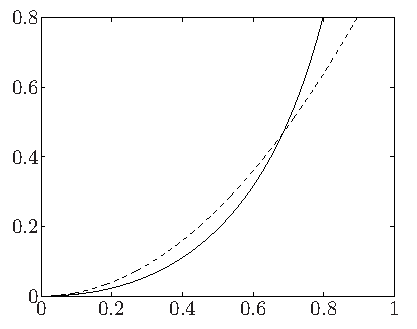
\includegraphics[width=.56\textwidth]{figures/ch09-later-24.pdf}
\caption*{图9.24 实线是函数 $-(\lambda+\log(1-\lambda))$，当 $\lambda$ 很小时，它近似为 $\lambda^2/2$。虚线为 $\lambda^2$，在区间 $0\le\lambda\le0.68$ 上是一个上界。}
\end{figure}
\subsection{自协调函数的牛顿法分析}
现在分析带回溯线搜索的牛顿法用于严格凸自协调函数 $f$ 时的情况。与前面一样，假设已知初始点 $x^{(0)}$，且下水平集 $S=\{x\mid f(x)\le f(x^{(0)})\}$ 闭。还假设 $f$ 有下界，这蕴含 $f$ 有最小点 $x^\star$，见习题9.19。

分析与第9.5.2节给出的经典分析十分相似，区别在于用自协调性代替强凸性与 Hessian 的 Lipschitz 条件作为基本假设，并且由牛顿减量代替梯度范数。我们将证明，存在仅依赖线搜索参数 $\alpha,\beta$ 的数 $\eta,\gamma>0$，且 $0<\eta\le1/4$，使以下结论成立。
\begin{itemize}
\item 若 $\lambda(x^{(k)})>\eta$，则
\begin{equation}
 f(x^{(k+1)})-f(x^{(k)})\le-\gamma.\tag{9.51}
\end{equation}
\item 若 $\lambda(x^{(k)})\le\eta$，则回溯线搜索选取 $t=1$，且
\begin{equation}
 2\lambda(x^{(k+1)})\le\bigl(2\lambda(x^{(k)})\bigr)^2.\tag{9.52}
\end{equation}
\end{itemize}
这些分别对应 (9.32) 和 (9.33)。与第9.5.3节一样，可递推应用第二个条件，得出对所有 $l\ge k$ 均有 $\lambda(x^{(l)})\le\eta$，且
\[
 2\lambda(x^{(l)})\le\bigl(2\lambda(x^{(k)})\bigr)^{2^{l-k}}
 \le(2\eta)^{2^{l-k}}\le\left(\frac12\right)^{2^{l-k}}.
\]
因此，对所有 $l\ge k$，
\[
 f(x^{(l)})-p^\star\le\lambda(x^{(l)})^2
 \le\frac14\left(\frac12\right)^{2^{l-k+1}}
 \le\left(\frac12\right)^{2^{l-k+1}},
\]
% Source PDF page 518 (printed p. 504)
所以，当 $l-k\ge\log_2\log_2(1/\epsilon)$ 时，有 $f(x^{(l)})-p^\star\le\epsilon$。

第一个不等式意味着，阻尼阶段所需步数不会超过 $(f(x^{(0)})-p^\star)/\gamma$。因此，从点 $x^{(0)}$ 出发，达到精度 $f(x)-p^\star\le\epsilon$ 所需的总迭代次数，以
\begin{equation}
 \frac{f(x^{(0)})-p^\star}{\gamma}+\log_2\log_2(1/\epsilon)\tag{9.53}
\end{equation}
为上界。这对应于牛顿法经典分析中的界 (9.36)。

\subsubsection*{阻尼牛顿阶段}
令 $\widetilde f(t)=f(x+t\Delta x_{\mathrm{nt}})$，则
\[
 \widetilde f'(0)=-\lambda(x)^2,\qquad
 \widetilde f''(0)=\lambda(x)^2.
\]
对 (9.46) 中的上界积分两次，得到 $\widetilde f(t)$ 的上界：
\begin{equation}
\begin{aligned}
 \widetilde f(t)&\le\widetilde f(0)+t\widetilde f'(0)-t\widetilde f''(0)^{1/2}
 -\log\bigl(1-t\widetilde f''(0)^{1/2}\bigr)\\
 &=\widetilde f(0)-t\lambda(x)^2-t\lambda(x)-\log(1-t\lambda(x)),
\end{aligned}\tag{9.54}
\end{equation}
在 $0\le t<1/\lambda(x)$ 时成立。

利用这个界，可以证明回溯线搜索总能给出步长 $t\ge\beta/(1+\lambda(x))$。为此，注意 $\hat t=1/(1+\lambda(x))$ 满足线搜索的退出条件：
\[
\begin{aligned}
 \widetilde f(\hat t)&\le\widetilde f(0)-\hat t\lambda(x)^2-\hat t\lambda(x)
 -\log(1-\hat t\lambda(x))\\
 &=\widetilde f(0)-\lambda(x)+\log(1+\lambda(x))\\
 &\le\widetilde f(0)-\alpha\frac{\lambda(x)^2}{1+\lambda(x)}\\
 &=\widetilde f(0)-\alpha\lambda(x)^2\hat t.
\end{aligned}
\]
第二个不等式来自对 $x\ge0$ 成立的事实
\[
 -x+\log(1+x)+\frac{x^2}{2(1+x)}\le0.
\]
由于 $t\ge\beta/(1+\lambda(x))$，有
\[
 \widetilde f(t)-\widetilde f(0)\le-\alpha\beta\frac{\lambda(x)^2}{1+\lambda(x)},
\]
因此 (9.51) 在
\[
 \gamma=\alpha\beta\frac{\eta^2}{1+\eta}
\]
时成立。

% Source PDF page 519 (printed p. 505)
\subsubsection*{二次收敛阶段}
我们将证明，可以取
\[
 \eta=(1-2\alpha)/4,
\]
它满足 $0<\eta<1/4$，因为 $0<\alpha<1/2$。也就是说，若 $\lambda(x^{(k)})\le(1-2\alpha)/4$，则回溯线搜索接受单位步长，并且 (9.52) 成立。

首先注意，上界 (9.54) 意味着，当 $\lambda(x)<1$ 时，单位步长 $t=1$ 得到的点位于 $\dom f$ 中。而且，若 $\lambda(x)\le(1-2\alpha)/2$，利用 (9.54)，有
\[
\begin{aligned}
 \widetilde f(1)&\le\widetilde f(0)-\lambda(x)^2-\lambda(x)-\log(1-\lambda(x))\\
 &\le\widetilde f(0)-\tfrac12\lambda(x)^2+\lambda(x)^3\\
 &\le\widetilde f(0)-\alpha\lambda(x)^2,
\end{aligned}
\]
因此单位步长满足充分下降条件。第二行来自：当 $0\le x\le0.81$ 时，$-x-\log(1-x)\le\tfrac12x^2+x^3$。

不等式 (9.52) 来自习题9.18中证明的下述事实：若 $\lambda(x)<1$，且 $x^+=x-\nabla^2f(x)^{-1}\nabla f(x)$，则
\begin{equation}
 \lambda(x^+)\le\frac{\lambda(x)^2}{(1-\lambda(x))^2}.\tag{9.55}
\end{equation}
特别地，若 $\lambda(x)\le1/4$，则
\[
 \lambda(x^+)\le2\lambda(x)^2,
\]
这就证明，当 $\lambda(x^{(k)})\le\eta$ 时，(9.52) 成立。

\subsubsection*{最终的复杂度界}
综合以上结果，牛顿迭代次数的界 (9.53) 成为
\begin{equation}
\begin{aligned}
 \frac{f(x^{(0)})-p^\star}{\gamma}+\log_2\log_2(1/\epsilon)
 ={}&\frac{20-8\alpha}{\alpha\beta(1-2\alpha)^2}
 \bigl(f(x^{(0)})-p^\star\bigr)\\
 &+\log_2\log_2(1/\epsilon).
\end{aligned}\tag{9.56}
\end{equation}
这一表达式只依赖线搜索参数 $\alpha,\beta$ 和最终精度 $\epsilon$。此外，涉及 $\epsilon$ 的项可以放心地用常数 $6$ 代替，因此这个界实际上只依赖 $\alpha,\beta$。对典型的 $\alpha,\beta$ 值，$f(x^{(0)})-p^\star$ 前面的系数大约为几百。例如，$\alpha=0.1$、$\beta=0.8$ 时，系数为 $375$。取容差 $\epsilon=10^{-10}$，得到界
\begin{equation}
 375\bigl(f(x^{(0)})-p^\star\bigr)+6.\tag{9.57}
\end{equation}
我们将看到，这个界相当保守，但它确实反映了所需牛顿步数的最坏值所呈现的一般形式。更精细的分析，例如 Nesterov 和 Nemirovski 最初给出的分析，可得到类似的界，但 $f(x^{(0)})-p^\star$ 前面的系数明显更小。

% Source PDF page 520 (printed p. 506)
\begin{figure}[htbp]\centering
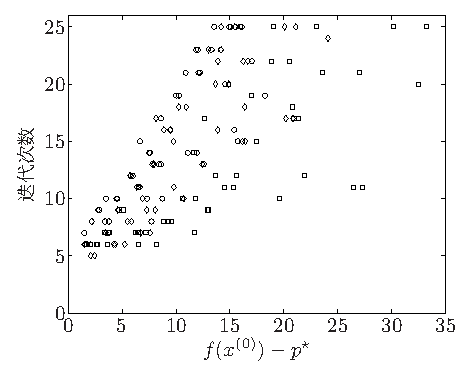
\includegraphics[width=.62\textwidth]{figures/ch09-later-25.pdf}
\caption*{图9.25 最小化自协调函数所需的牛顿迭代次数与 $f(x^{(0)})-p^\star$ 的关系。函数形式为 $f(x)=-\sum_{i=1}^m\log(b_i-a_i^\T x)$，问题数据 $a_i,b$ 随机生成。圆圈表示 $m=100,n=50$ 的问题，方框表示 $m=1000,n=500$ 的问题，菱形表示 $m=1000,n=50$ 的问题。每种问题各画出50个实例。}
\end{figure}
\subsection{讨论与数值例子}
\subsubsection*{一族自协调函数}
将上界 (9.57) 与最小化自协调函数实际所需的迭代次数进行比较，很有意思。考虑形如
\[
 f(x)=-\sum_{i=1}^m\log(b_i-a_i^\T x)
\]
的一族问题。

问题数据 $a_i,b$ 按以下方式生成。对每个问题实例，$a_i$ 的各分量由均值为零、方差为一的独立正态分布生成，$b$ 的各分量由 $[0,1]$ 上的均匀分布生成。剔除向下无界的问题实例。对每个问题，先计算 $x^\star$，再随机选择方向 $v$，取 $x^{(0)}=x^\star+sv$ 作为初始点，其中 $s$ 使 $f(x^{(0)})-p^\star$ 等于 $0$ 到 $35$ 之间的某个指定值。需要指出，$f(x^{(0)})-p^\star=10$ 或更大时，初始点实际上已经十分接近多面体边界。然后使用牛顿法最小化该函数，回溯线搜索参数取 $\alpha=0.1,\beta=0.8$，容差为 $\epsilon=10^{-10}$。

图9.25给出150个问题实例中，所需牛顿迭代次数与 $f(x^{(0)})-p^\star$ 的关系。圆圈表示 $m=100,n=50$ 的50个问题；方框表示 $m=1000,n=500$ 的50个问题；菱形表示 $m=1000,n=50$ 的50个问题。

% Source PDF page 521 (printed p. 507)
对这里所用的回溯参数，前面得到的复杂度界为
\begin{equation}
 375\bigl(f(x^{(0)})-p^\star\bigr)+6,\tag{9.58}
\end{equation}
显然远大于这150个实例实际所需的迭代次数。图中结果表明，可能存在一个形式相同的有效界，但 $f(x^{(0)})-p^\star$ 前面的常数小得多，例如约为 $1.5$。事实上，表达式
\[
 f(x^{(0)})-p^\star+6
\]
作为所需牛顿步数的粗略预测还不错，尽管它显然不是唯一因素。首先，有不少实例所需牛顿步数更少，可以猜测，它们对应比较“幸运”的初始点。还应注意，对于含500个变量的较大问题，即图中的方框，牛顿步数异常少的情形似乎更多。

这里需要说明，所研究的问题族不仅自协调，而且实际上是\emph{最小自协调}的，即当 $\alpha<1$ 时，$\alpha f$ 不自协调。因此，不能简单地缩放 $f$ 来改进界 (9.58)。函数 $f(x)=-20\log x$ 是自协调但并非最小自协调的例子，因为 $(1/20)f$ 也自协调。

\subsubsection*{自协调性在实际中的意义}
前面已经看到，对于强凸目标函数，牛顿法通常表现很好。这个概括性的说法可以通过经验结果支持，也可以通过牛顿法的经典分析来说明；经典分析给出了复杂度界，但它依赖几个几乎总是未知的常数。

对于自协调函数，我们能给出更明确的结论：复杂度界完全显式，不依赖任何未知常数。经验研究表明，这个界可以大幅收紧，但其一般形式，即一个小常数加上 $f(x^{(0)})-p^\star$ 的某个倍数，似乎至少能粗略预测最小化一个近似最小自协调函数所需的牛顿步数。

目前还不清楚，在实际中，牛顿法最小化自协调函数是否比最小化非自协调函数更容易；甚至还不清楚如何精确表述这一命题。目前能够说的是，与非自协调函数相比，自协调函数是一类能够对牛顿法复杂度作出更多明确论断的函数。
